\documentclass[11pt]{article}

\usepackage[portuguese]{babel}
\usepackage[utf8]{inputenc}
\usepackage{amsmath}
\usepackage{graphicx}
\usepackage{float}
\usepackage{subfig}
\usepackage{fixltx2e}
\usepackage[bottom]{footmisc}
\usepackage{color}
\usepackage{todonotes}
% \usepackage[usenames,dvipsnames]{xcolor}
\usepackage[font=footnotesize]{caption}

\usepackage{titlesec}
\setcounter{secnumdepth}{4}
\titleformat{\paragraph}
{\normalfont\normalsize\bfseries}{\theparagraph}{1em}{}
\titlespacing*{\paragraph}
{0pt}{3.25ex plus 1ex minus .2ex}{1.5ex plus .2ex}

\numberwithin{equation}{section}

\linespread{1.3}
\usepackage{indentfirst}
\usepackage[top=2cm, bottom=2cm, right=2.2cm, left=2.2cm]{geometry}
\addto\captionsportuguese{\renewcommand{\contentsname}{Índice}}

\begin{document}

\begin{titlepage}
\begin{center}

\hfill \break
\hfill \break


\includegraphics[width=0.3\textwidth]{./logo}~\\[1cm]

\textsc{\LARGE Instituto Superior Técnico}\\[0.25cm]
\textsc{\Large Mestrado Integrado em Engenharia Electrotécnica e de Computadores}\\[1.8cm]
\textsc{\huge Arquitecturas Avançadas de Computadores}\\[0.25cm]

{\huge \bfseries Simulação de um processador $\mu$Risc com funcionamento multi-ciclo\\[1.2cm]}

\begin{tabular}{ l l }
Guilherme Branco Teixeira & \hspace{2mm} n.º 70214 \\ 
Maria Margarida Dias dos Reis & \hspace{2mm} n.º 73099 \\
Nuno Miguel Rodrigues Machado & \hspace{2mm} n.º 74236 
\end{tabular}

\vfill

{\large Lisboa, 29 de Março 2014} 

\end{center}
\end{titlepage}
 
\pagenumbering{gobble}
\clearpage

\footnote{É de referir que as imagens e tabelas não foram colocadas em anexo de modo a permitir uma melhor compreensão do relatório.}

\tableofcontents
\pagebreak

\clearpage
\pagenumbering{arabic}

\section{Introdução}

Com este trabalho laboratorial pretende-se projectar um processador $\mu$Risc, de 16 \textit{bits} com arquitectura RISC, com um funcionamento multi-ciclo. O processador possui 8 registos de uso geral e 42 instruções, sendo que cada instrução demora quatro ciclos a completar, um ciclo por cada andar do processador. O processador é feito com recurso a uma linguagem de descrição de \textit{hardware} - VHDL.

\section{Características do Processador}

O processador elaborado foi simulado para uma placa Artix 7 e tem as seguintes características: 16 \textit{bits}; 8 registos de uso geral de 16 \textit{bits} de largura (R0, \ldots, R7); 42 instruções; instruções de 3 operandos; organização de dados na memória do tipo \textit{big endian}; uma memória ROM de 8 KBytes (4k endereços $\times$ 2 \textit{bytes}) endereçada com palavras de 12 \textit{bits} utilizada para as instruções/programa e uma memória RAM de 8 KBytes (4k endereços $\times$ 2 \textit{bytes}) endereçada com palavras de 12 \textit{bits} utilizada para os dados.

\section{Estrutura do Processador}

O processador $\mu$Risc que foi projectado encontra-se dividido em quatro andares - num primeiro andar é feito o \textit{instruction fetch} (IF), no segundo andar é feito o \textit{instruction decode} (ID) e o \textit{operand fetch} (OF), no terceiro andar são executadas operações da ALU (EX) e de acesso à memória de dados (MEM) e, por fim, no quarto e último andar é feita a escrita no banco de registos, o \textit{write back} (WB).

\subsection{Primeiro Andar - IF}

No primeiro andar obtem-se a instrução a ser executada a cada ciclo. Como todas as instruções do programa são armazenadas na memória ROM, o \textit{instruction fetch} tem a função de endereçar a ROM com o \textit{program counter} (\texttt{PC}) e ler a instrução desse endereço.

FIGURA 1

O \textit{instruction fetch} é simplesmente um somador que, em cada ciclo, soma \texttt{1} ao endereço actual e armazena o resultado no registo \texttt{PC}, como se pode ver na Figura 1. O endereço actual, além de ser um operando do somador, também endereça a memória ROM.

Podem ocorrer duas situações que alteram o funcionamento sequencial do \textit{instruction fetch} - a primeira ocorre quando há uma transferência de controlo do tipo condicional ou incondicional, seleccionando o sinal \texttt{destino\_cond} no \texttt{MUX\_1} e o resultado do somador no \texttt{MUX\_2}, ou seja, o sinal \texttt{s\_cond} está a \textit{high} e \texttt{s\_jump} a \textit{low}. A última situação ocorre quando existe uma transferência de controlo do tipo \textit{jump and link} ou \textit{jump register}, selecionando o sinal \texttt{destino\_jump} no \texttt{MUX\_2}, ou seja, o sinal \texttt{s\_jump} está a \textit{high}.

\todo{se calhar e melhor explicar o significado destes sinais}

\begin{table}[h]
	\centering
	\caption{Caracterização do registo de saída do andar de \textit{instruction fecth}.}
	\vspace{-2mm}
 	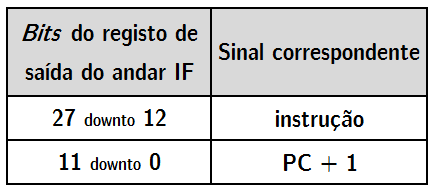
\includegraphics[keepaspectratio=true, scale=0.35]{tabelas/regIF}
\end{table}

\subsection{Segundo Andar - ID e OF}

\subsubsection{ID}

No segundo andar é realizada a descodificação da instrução a ser executada, sendo a principal descodificação feita neste andar, com um só sinal descodificado no último, que será explicado mais à frente no relatório.

\begin{figure}[H]
	\centering
	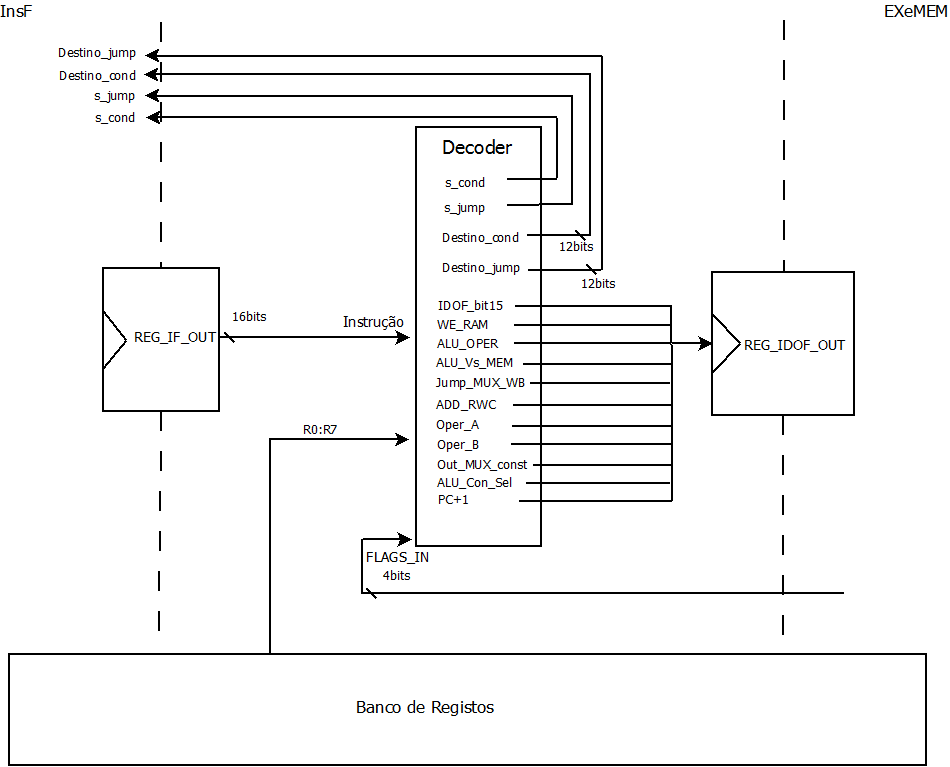
\includegraphics[keepaspectratio=true, scale=0.5]{imagens/idof}
	\caption{Selecção dos operando \texttt{A} e \texttt{B}.}
	\vspace{-0.8em}
\end{figure}

Analisando a figura anterior, existe três grupos de sinais de entrada.

\vspace{-2mm}

\begin{itemize}
	\item  O sinal \texttt{instrução} proveniente do primeiro andar, \textit{instruction fetch}, é um sinal de 16 \textit{bits} que representa a instrução a ser descodificada;
	\vspace{-2.5mm}
	\item Os sinais \texttt{R0} \ldots \texttt{R7}, provenientes do banco de registos, devolvem o valor do registo respectivo, sendo posteriormente selecionados os registos indicado pela instrução para operandos;
	\vspace{-2.5mm}
	\item  O sinal \texttt{FLAGS\_IN} é o resultado da actualização das \textit{flags} realizado no terceiro andar.
\end{itemize}

Os sinais de saída do descodificador são distribuídos pelos 4 andares do processador, como se verá.
	
\paragraph{Sinais de controlo para o primeiro andar - IF} 

Os sinais de controlo para o primeiro andar são referentes às instruções do tipo de transferência de controlo. Há dois tipos principais de operações - salto relativo ao \texttt{PC + 1} ou salto absoluto. 

Para poder haver um salto é necessário detectar se a instrução é do tipo de transferência de controlo e, com essa ideia em mente, foi criado o sinal auxiliar \texttt{Active\_FlagTest}. A figura abaixo mostra a função lógica de verificação. 

\vspace{2mm}

\begin{figure}[H]
	\centering
	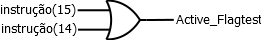
\includegraphics[keepaspectratio=true, scale=0.55]{imagens/active_flagtest}
	\caption{Construção do sinal Active\_Flagteste}
	\vspace{-0.8em}
\end{figure}
De seguida, é preciso saber qual o tipo de salto a ser executado. 

\vspace{2mm}

\begin{figure}[H]
	\centering
	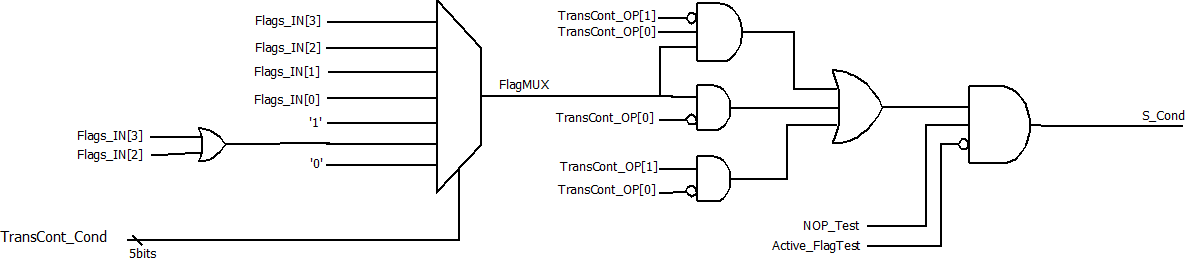
\includegraphics[keepaspectratio=true, scale=0.4]{imagens/Flagteste}
	\caption{Selecção da constante a carregar.}
	\vspace{-0.8em}
\end{figure}

A figura anterior representa a função lógica do sinal \texttt{s\_cond} que controla o salto relativo ao \texttt{PC + 1}. É  de referir que o sinal \texttt{TransCont\_OP} corresponde aos \textit{bits} \texttt{12} e \texttt{13} da instrução, ou seja, é um sinal de 2 \textit{bits} que identifica as operações de transfêrencia de controlo. O sinal \texttt{TransCont\_Cond} corresponde aos \textit{bits} \texttt{8} a \texttt{11}, ou seja, é um sinal de 4 \textit{bits} que identifica qual a \textit{flag} a ser testada.

Há três tipos diferentes de operações em que pode ocorrer este tipo de salto.

\begin{itemize}
	\item Quando há um \textit{jump} incondicional: \texttt{TransCont\_OP = "10"}, \texttt{Active\_FlagTest = 0} e \texttt{NOP\_Test = 1};
	\vspace{-2.5mm}
	\item Quando há um \textit{jump false}: \texttt{TransCont\_OP = "00"}, \texttt{Active\_FlagTest = 0}, \texttt{NOP\_Test = 1} e o resultado do MUX de 8:1 é \textit{false}, ou seja, a \textit{flag} escolhida do registo \texttt{MSR} é \textit{false};
	\vspace{-2.5mm}
	\item Quando há um \textit{jump true}: \texttt{TransCont\_OP = "00"}, \texttt{Active\_FlagTest = 0}, \texttt{NOP\_Test = 1} e o resultado do MUX de 8:1 é \textit{true}, ou seja, a \textit{flag} escolhida do registo \textit{MSR} é \textit{true}.
\end{itemize}

\begin{figure}[H]
	\centering
	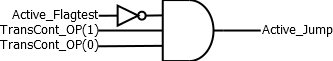
\includegraphics[keepaspectratio=true, scale=0.55]{imagens/activejump}
	\caption{Selecção da constante a carregar.}
	\vspace{-0.8em}
\end{figure}

A figura anterior representa a função lógica do sinal \texttt{s\_jump} que controla o salto absoluto. O sinal \texttt{s\_jump} é activado, \texttt{s\_jump = 1}, quando \texttt{active\_FlagTest = 0} e o \texttt{TransCont\_OP = "11"}.
 	
\paragraph{Sinais de controlo para o segundo andar - ID e OF}

Os sinais de controlo para o segundo andar são referentes ao controlo do \textit{operand fetch}. Para que o \textit{operand fetch} defina os operandos A e B é necessário identificar os endereços desses operandos.

O sinal \texttt{ADD\_RA\_C} define o endereço do operando \texttt{A}. Como a instrução do tipo constantes reutiliza o endereço de escrita como leitura, \texttt{ADD\_RWC}, é necessário acrescentar lógica para poder resolver o problema destas operações. A solução encontrada foi utilizar um MUX de 2:1 de forma a escolher o endereço \texttt{ADD\_RA} (sinal de 3 \textit{bits} que é igual ao sinal \texttt{instrução(5 {\footnotesize downto} 3)}) ou \texttt{ADD\_RWC} (sinal de 3 \textit{bits} que é igual ao sinal \texttt{instrução(13 {\footnotesize downto} 11)}). A figura abaixo define como se obtém o endereço.

\begin{figure}[H]
	\centering
	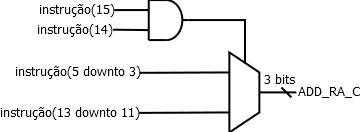
\includegraphics[keepaspectratio=true, scale=0.6]{imagens/ADD_RA_C}
	\caption{Mux que permite selecionar}
	\vspace{-0.8em}
\end{figure}

O sinal \texttt{ADD\_RB} (sinal de 3 \textit{bits} que é igual ao sinal \texttt{instrução(2 {\footnotesize downto} 0)}) é simplesmente o endereço do registo para obter o operando \texttt{B}. 

O sinal \texttt{select\_mux\_constantes} (sinal com dimensão de 2 \textit{bits}) é o \textit{bit} \texttt{15} do sinal \texttt{instrução}  concatenado com o \textit{bit} \texttt{10} do mesmo sinal. Este sinal tem a função de selecionar se a operação de constantes é do tipo \textit{lcl}, \texttt{select\_mux\_constantes = "10"}, do tipo \textit{lch}, \texttt{select\_mux\_constantes = "11"} ou um carregamento directo de uma constante de 11 \textit{bits} com o \textit{bit} de sinal replicado, \texttt{select\_mux\_constantes = "00"} e \texttt{select\_mux\_constantes = "01"}. 

\paragraph{Sinais de controlo para o terceiro andar - EX e MEM}
WE\_RAM ALU\_OPER ALU\_VS\_MEM 


\paragraph{Sinais de controlo para o quarto andar - WB}
IDOF\_bit15 ALU\_Con\_Sel ADD\_RWC PC+1
	
\todo{LEGENDAS BOAS}

\todo{explicar WE da RAM, que eu depois uso quando explico a MEM. nao esta no desenho do decoder?}

\subsubsection{OF}

É também no segundo andar que é feito o \textit{operand fetch}. Numa primeira fase é preciso definir os operandos \texttt{A} e \texttt{B} da ALU, feito de acordo com a seguinte lógica.

\begin{figure}[H]
	\centering
	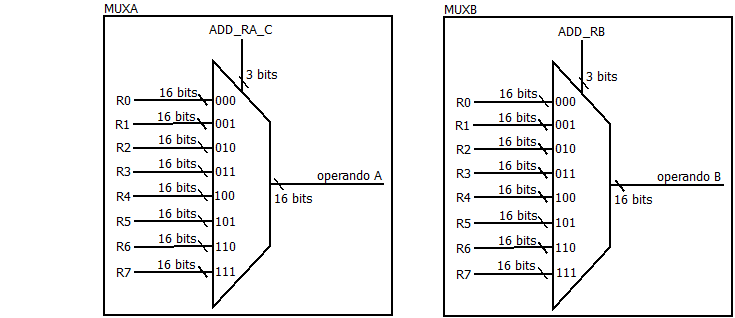
\includegraphics[keepaspectratio=true, scale=0.6]{imagens/OF1}
	\caption{Selecção dos operando \texttt{A} e \texttt{B}.}
	\vspace{-0.8em}
\end{figure}

Para fazer a selecção é necessário recorrer a alguns sinais que o \textit{decoder} explicado anteriormente fornece - \texttt{ADD\_RA\_C} (sinal 3 \textit{bits} que permite fazer a selecção do operando \texttt{A} no \texttt{MUXA}) e \texttt{ADD\_RB} (sinal 3 \textit{bits} que permite fazer a selecção do operando \texttt{B} no \texttt{MUXB}). 

Os sinais que definem o operando \texttt{A} e o operando \texttt{B} são depois passados para o terceiro andar para que a ALU possa fazer operações com o seu valor.

É também aqui que se faz a selecção das constantes que depois serão carregadas nos registos do banco de registos, algo que é feito de acordo com a próxima figura.

\vspace{-2.1mm}

\begin{figure}[H]
	\centering
	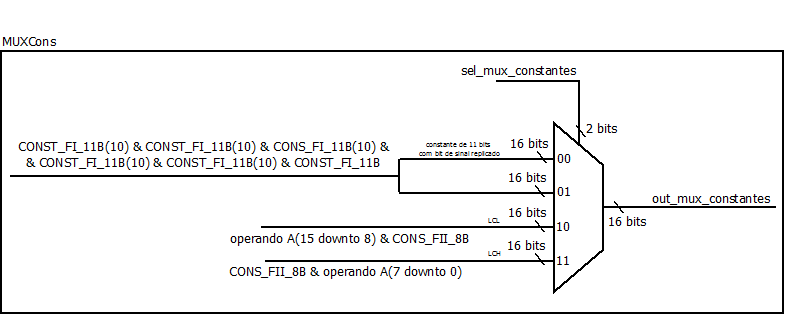
\includegraphics[keepaspectratio=true, scale=0.55]{imagens/OF2}
	\caption{Selecção da constante a carregar.}
	\vspace{-0.8em}
\end{figure}

Do \textit{decoder} são fornecidos os seguintes sinais - \texttt{CONS\_FI\_11B} (constante de 11 \textit{bits} que é carregada directamente), \texttt{CONS\_FII\_8B} (constante de 8 \textit{bits} com que é feita uma operação de \textit{lch} ou \textit{lcl}) e \texttt{select\_mux\_constantes} \todo{este sinal nao esta no decoder?} (sinal de 2 \textit{bits} que permite fazer a selecção dos três casos definidos anteriormente no \texttt{MUXCons}).

De referir que, \todo{explicar que não faço ands, é so fios}

\begin{table}[h]
	\centering
	\caption{Caracterização do registo de saída do andar de \textit{instruction decoding} e \textit{operand fetch}.}
	\vspace{-2mm}
 	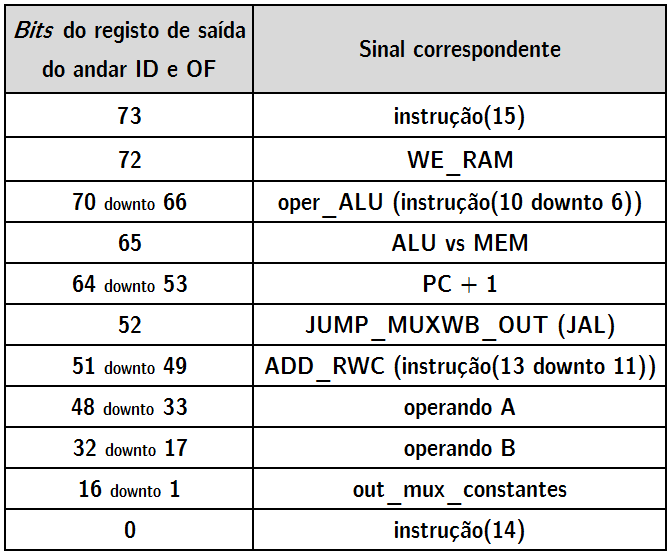
\includegraphics[keepaspectratio=true, scale=0.45]{tabelas/regIDOF}
\end{table}

\subsection{Terceiro Andar - EX e MEM}

Neste andar trata-se de executar operações da ALU bem com operações da memória, sendo que, ao contrário do MIPS, em que é possível utilizar a ALU e a memória na mesma instrução, no processador $\mu$Risc projectado tal não é possível. A memória RAM está colocada no mesmo andar que a execução porque não é necessário fazer cálculos dos endereços, se tal fosse necessário, a memória teria de estar no andar seguinte àquele que contém a ALU. 

\subsubsection{ALU (EX)}

No terceiro andar o bloco da ALU é responsável pelas operações aritméticas e lógicas. Este bloco recebe como entrada os sinais dos operandos \texttt{A} e \texttt{B}, um sinal de 4 \textit{bits} com as \textit{flags} actuais para posterior actualização, se for esse o caso, e também um sinal de 5 \textit{bits} que representa a operação que a ALU vai efectuar. Como saída tem-se um sinal de 16 \textit{bits} que representa o resultado da ALU e um sinal de 4 \textit{bits} que representa as \textit{flags}.

Analisando primeiramente as seis operações aritméticas a realizar concluiu-se que algumas podiam ser simplificadas de modo a que todas pudessem ser efectuadas com recurso a apenas um somador. A seguinte tabela demonstra como todas as operações aritméticas a realizar podem ser calculadas apenas com um somador.

\begin{table}[h]
	\centering
	\caption{Caracterização somador utilizado nas operações aritméticas.}
	\vspace{-2mm}
 	\includegraphics[keepaspectratio=true, scale=0.35]{tabelas/adder}
\end{table}

Esta solução é mais eficiente pois os somadores têm um tempo de propagação elevado. As seis operações aritméticas podem ser feitas usando um somador com \textit{carry-in}, que efectua o seguinte cálculo: \texttt{out\_ARI} $=$ \texttt{P} + \texttt{Q} + \texttt{cIN}. 

O operando \texttt{P} corresponde sempre ao operando \texttt{A}, o operando \texttt{Q} corresponde a  um sinal diferente dependendo da operação aritmética a realizar, tal como o \textit{carry-in} que é usado para operações como incrementos, podendo também completar o \texttt{!B} em complemento para dois. Os dois sinais de entrada do somador recebem uma concatenação com o bit \texttt{0} como o bit mais significativo, sendo isto feito para que a saída do somador tenha 17 \textit{bits}, tornando possível a actualização da \textit{flag} de \textit{cary}. Este somador foi projectado tal como representado na figura abaixo.

\vspace{1mm}

\begin{figure}[H]
	\centering
	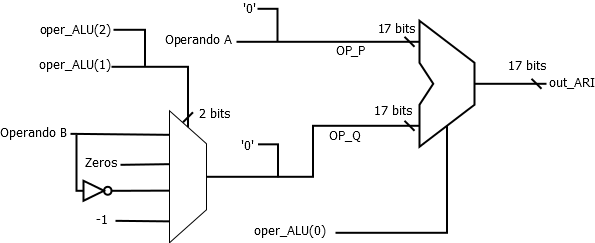
\includegraphics[keepaspectratio=true, scale=0.55]{imagens/Arit}
	\caption{Esquema do bloco aritmético da ALU.}
	\vspace{-0.8em}
\end{figure}

No caso das operações de \textit{shift}, tal como nas operações aritméticas, a saída é representada com 17 \textit{bits}, pela mesma razão do \textit{cary}. Para escolher entre as operações de \textit{shift} é usado um MUX de 2:1 tal como está \textit{pseudo}-representado na figura.

\begin{figure}[H]
	\centering
	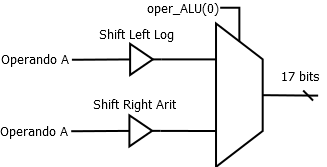
\includegraphics[keepaspectratio=true, scale=0.55]{imagens/Shift}
	\caption{Esquema do bloco de operações de \textit{shift} da ALU.}
	\vspace{-0.8em}
\end{figure}

No caso das operações lógicas, que representam 16 operações, fez-se um esforço para reduzir um MUX de 16:1 para um MUX de 8:1 devido à diferença de tempo gasto entre os dois MUXs. Após uma análise cuidada das operações a realizar, foi possível establecer uma relação entre as operações, tal como se pode observar na tabela abaixo.

\begin{table}[h]
	\centering
	\caption{Descrição das operações lógicas a realizar.}
	\vspace{-2mm}
 	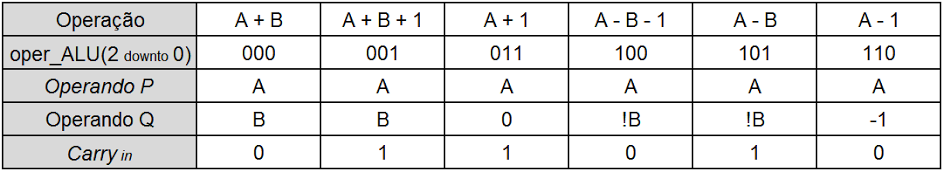
\includegraphics[keepaspectratio=true, scale=0.35]{tabelas/MUX8-1}
\end{table}

Ao observar o sinal \texttt{oper\_ALU(2 {\footnotesize downto} 0)} e as suas operações podemos perceber que quando temos um valor específico de \texttt{oper\_ALU(2 {\footnotesize downto} 0)} com a sua respectiva operação, o valor negado desse valor representa a negação da operação. Podendo assim criar um mux apenas com 8 entradas entradas e com um sinal de selecção que permite selecionar a operação X quando de facto desejamos a operação !X, como representa a seguinte figura.

\vspace{1mm}

\begin{figure}[H]
	\centering
	\includegraphics[keepaspectratio=true, scale=0.55]{imagens/Log}
	\caption{Esquema do bloco de operações lógicas da ALU.}
	\vspace{-0.8em}
\end{figure}

Será no entanto, quando necessário, negar a operação, esta negação será efectuada no mux final da ALU como demonstrado na figura %refrenciar a figura assinalada.

De notar que a saída das operações lógicas necessita apenas de 16 \textit{bits} e não 17 pois uma operação lógica não produz \textit{carry}.

Finalmente, após a verificação das \textit{flags}, tem-se um MUX de 4:1, onde as entradas de 17 \textit{bits} são reduzidas para 16 \textit{bits}, retirando-lhes o \textit{bit} mais significativo que, relembre-se, tinha como objectivo a verificação da flag de \textit{cary}. A saída deste MUX é um sinal de 16 \textit{bits} que representa o resultado da operação da ALU, tal como se pode verificar na figura seguinte.

Na Figura \ref{fig:ALU} encontra-se um esquema completo da ALU.

\begin{figure}[H]
	\centering
	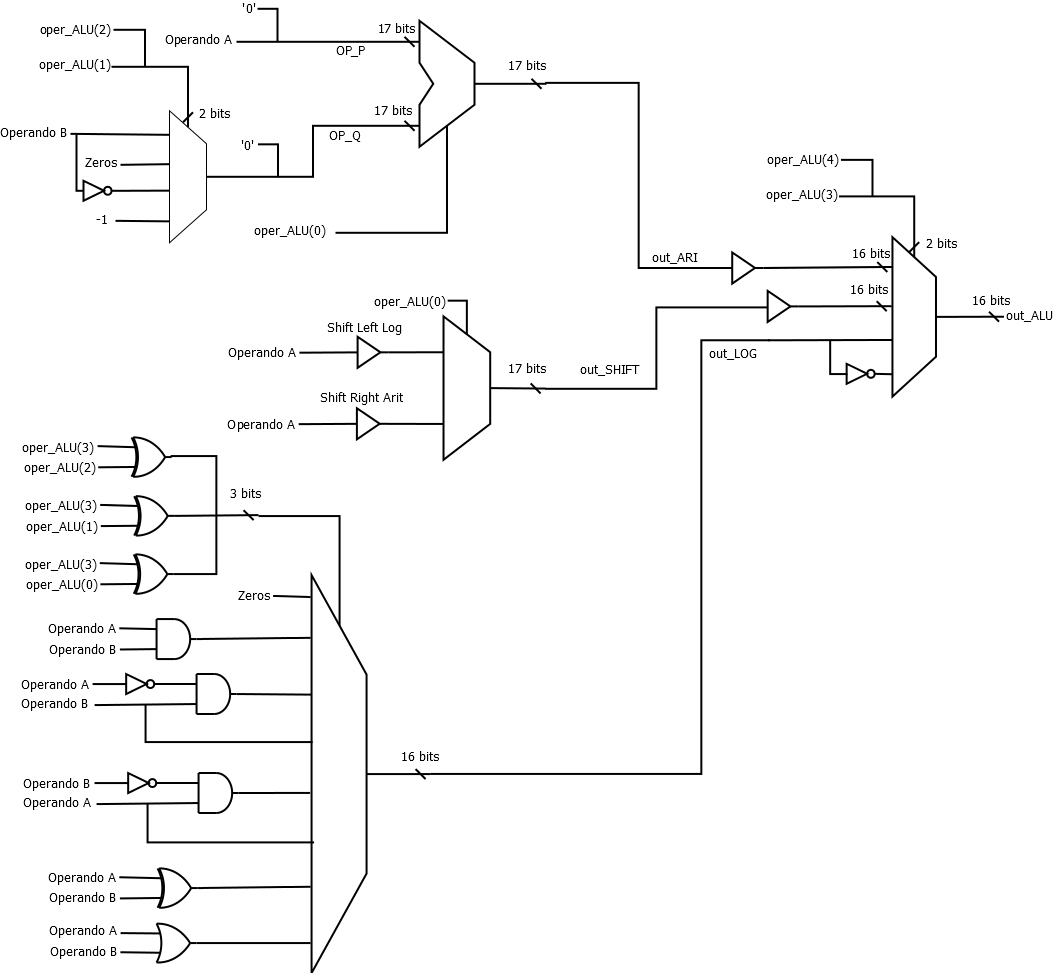
\includegraphics[keepaspectratio=true, scale=0.475]{imagens/ALU}
	\caption{Esquema do bloco de operações lógicas da ALU.}
	\vspace{-0.8em}
	\label{fig:ALU}
\end{figure}

Para cada um dos três sinais de saída (\texttt{out\_ARI}, \texttt{out\_SHIFT} e \texttt{out\_LOG}) é criado um sinal que corresponde às \textit{flags} que cada operação pode actualizar. No caso das operações aritméticas é criado um sinal de 4 \textit{bits} com as quatro \textit{flags} atualizadas indiscriminadamente. No caso das operações de \textit{shift} é criado um sinal de 3 \textit{bits} apenas pois, as \textit{flags} que podem vir a ser actualizadas nessas duas operações, são a flag de \texttt{Zero}, de \texttt{Negative} e de \texttt{Carry}. No caso das operações lógicas é criado um sinal com apenas dois \textit{bits} que representam as \textit{flags} que poderão ser atualizadas neste tipo de operações, a \textit{flag} de \texttt{Zero} e de \texttt{Negative}.

Estes três sinais criados serão utilizados no bloco de actualização de \textit{flags}, tal como explicado na secção ~\ref{subsec:act-flags}.

\subsubsection{Actualização das \textit{Flags}}
\label{subsec:act-flags}

Este bloco recebe como entrada o sinal de 4 \textit{bits} que representa as \textit{flags} da operação realizada na instrução anterior, os três sinais criados na ALU que representam as \textit{flags} atualizadas indiscriminadamente e também o sinal de 5 \textit{bits} que representa a operação que a ALU efectuou de modo a que seja possível discriminar que \textit{flags} actualizar. A saída é um sinal de 4 \textit{bits} que representa as \textit{flags} atualizadas discriminadamente.

Ao analisar o quadro de operações da ALU, é possível reparar que existem apenas quatro tipos de atualizações de \textit{flags}:

\vspace{-2mm}

\begin{itemize}
  \item Nenhuma;
  \vspace{-2.5mm}
  \item \texttt{Zero} e \texttt{Negative};
  \vspace{-2.5mm}
  \item \texttt{Zero}, \texttt{Negative} e \texttt{Carry};
  \vspace{-2.5mm}
  \item \texttt{Zero}, \texttt{Negative}, \texttt{Carry} e \texttt{Overflow} (Todas).
\end{itemize}

Foi então criado um sinal que tem como objectivo discernir de entre todas as \textit{flags} quais a actualizar. Este sinal foi criado com a lógica representada na seguinte figura.

\begin{figure}[H]
	\centering
	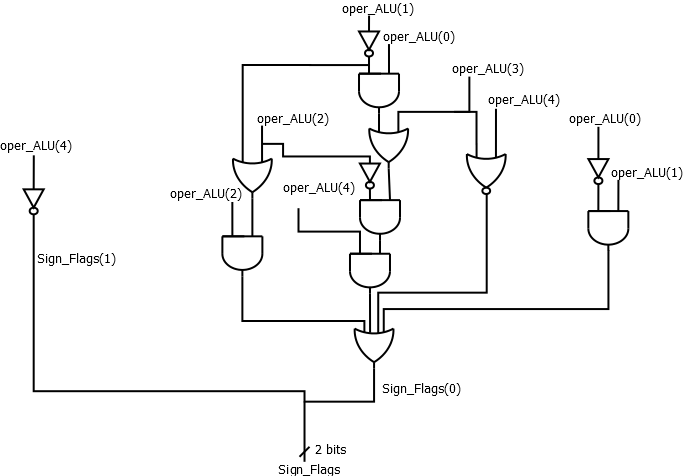
\includegraphics[keepaspectratio=true, scale=0.5]{imagens/Sign_Flags}
	\caption{Lógica que calcula o sinal de selecção de quais as \textit{flags} a actualizar.}
	\vspace{-0.8em}
\end{figure}

Com o sinal \texttt{Sign\_Flags} como sinal de selecção é então possível criar um MUX de 2:1 que tem em cada entrada o que está descrito na seguinte tabela.

\vspace{1.5mm}
\begin{table}[h]
	\centering
	\caption{Actualização de \textit{flags} consoante a operação realizada.}
	\vspace{-2mm}
 	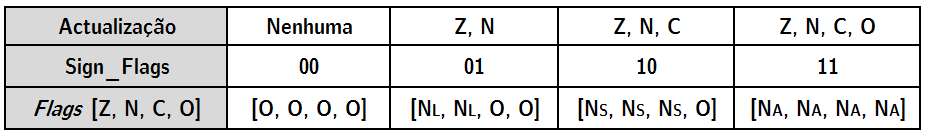
\includegraphics[keepaspectratio=true, scale=0.45]{tabelas/tabelaFlags}
\end{table}

Onde \texttt{O} representa um bit de \textit{flags} não actualizado, e \texttt{N{\scriptsize {L,S,A}}} representa um novo \textit{bit} actualizado retirado do sinal de entrada referente às operações lógicas, de \textit{shift} ou aritméticas. Dependendo de \texttt{Sign\_Flags} tem-se actualizações diferentes nas \textit{flags}, podendo assim ter uma saída do MUX que será também a saída deste bloco de atualização das \textit{flags}.

\subsubsection{MEM}

Relativamente às operações de memória é necessário tratar de \textit{loads} e \textit{stores}. Em ambos os casos o endereçamento à RAM é feito com o valor guardado no registo \texttt{A}, especificado pelos \textit{bits} \texttt{3} a \texttt{5} da instrução. Para o caso de um \textit{load} o valor que estiver nessa posição de memória é guardado no registo \texttt{WC}, especificado pelo \textit{bits} \texttt{11} a \texttt{13} da instrução, estando o \textit{write enable} da RAM a \textit{low}. Para o caso de um \textit{store} pretende-se escrever o conteúdo do registo \texttt{B}, especificado pelos \textit{bits} \texttt{0} a \texttt{2} da instrução, na posição de memória anteriormente endereçada, sendo necessário colocar o \textit{write enable} da RAM a \textit{high}. 

Uma vez que o conteúdo dos registos é de 16 \textit{bits}, para endereçar a memória RAM recorre-se apenas ao 12 menos significativos. O sinal de \textit{write enable} da RAM é, como já se viu, calculado no andar anterior, mas só neste terceiro andar é que é ligado à RAM. Optou-se por fazer desta maneira pois o cálculo desse sinal depende apenas de \textit{bits} específicos da instrução, como se pode ver na Figura TAL, fazendo então parte do andar que trata de fazer o \textit{decoding} da instrução.

É também neste andar que se liga a saída de dados da RAM ao sinal que depois será escrito no registo \texttt{WC} do banco de registos (para o caso do \textit{load}) e liga-se também o valor que estiver no registo \texttt{B} à entrada de dados da RAM, para que depois possa ser escrito na posição de memória especificada (para o caso do \textit{store}).

De referir que as leituras da RAM são feitas assincronamente e as escritas são feitas nos flancos positivos de relógio.

Na figura apresentada de seguida encontra-se o esquema de acesso à memória RAM.

\begin{figure}[H]
	\centering
	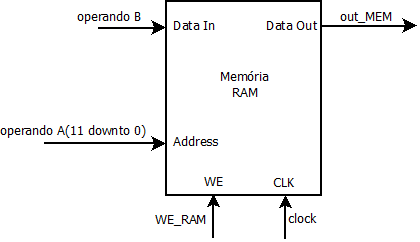
\includegraphics[keepaspectratio=true, scale=0.55]{imagens/RAM}
	\caption{Representação da memória de dados, RAM.}
	\vspace{-0.8em}
\end{figure}

Na tabela abaixo está a descrição do registo de saída deste andar.

\begin{table}[h]
	\centering
	\caption{Caracterização do registo de saída do andar de \textit{execute} e \textit{memory access}.}
	\vspace{-2mm}
 	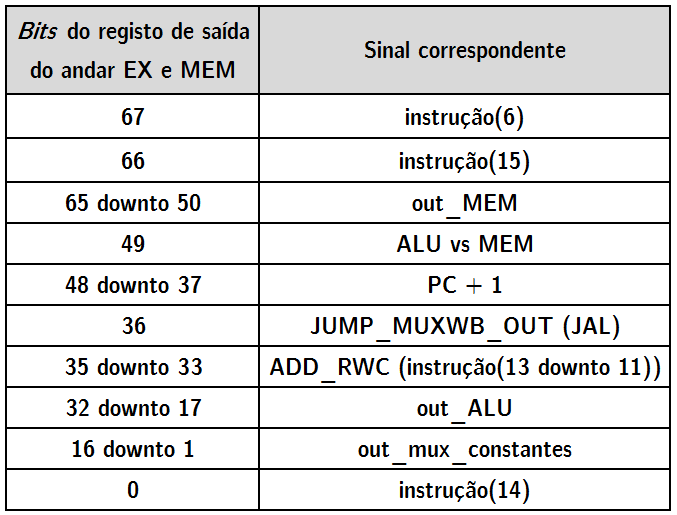
\includegraphics[keepaspectratio=true, scale=0.45]{tabelas/regEXMEM}
\end{table}

\subsection{Quarto Andar - WB}

No último andar os diversos resultados possíveis são escritos no banco de registos - pode ser o resultado de uma operação da ALU, o resultado de uma operação sobre a memória (\textit{load}), o carregamento de uma constante ou guardar em \texttt{R7} o valor do próximo \textit{program counter}. Como se pode ver na figura seguinte, a seleção de qual os resultados deve ser escrito é feita com recurso a um MUX de 4:1. 

\begin{figure}[h]
	\centering
	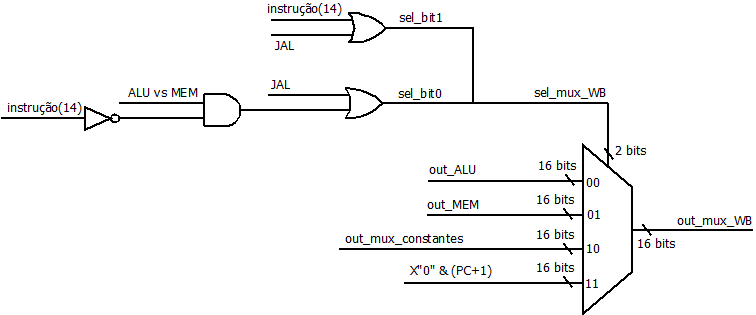
\includegraphics[keepaspectratio=true, scale=0.5]{imagens/WB1}
	\caption{MUX para selecção do que vai ser escrito num dos registos do banco de registos.}
	\vspace{-0.8em}
\end{figure}

Uma vez seleccionado o resultado a escrever é preciso escolher qual o registo onde se pretende escrever esse mesmo resultado, o registo \texttt{WC}. 

Para instruções da ALU a escolha do registo onde se quer escrever o resultado final é feita com recurso aos \textit{bits} \texttt{11} a \texttt{13} da instrução, assim como para operações de carregamento de constantes. Originalmente pensou-se em utilizar os 3 \textit{bits} referidos anteriormente para controlar um MUX de 8:1 que colocasse a \textit{high} um dos 8 \textit{enables} (que estão armazenados nos 8 \textit{bits} de um vector).

Relativamente à escrita no registo \texttt{R7} para quando se está numa operação de \textit{jump and link}, verifica-se, com recurso a uma porta AND, quando é que o sinal de selecção do MUX de 4:1 está a \texttt{11}, ou seja, quando se vai escrever num dos registos o valor de \texttt{PC} $+$ 1, e coloca-se o sinal de selecção do MUX de 8:1 com o valor \texttt{111}, ou seja, apenas o enable de \texttt{R7} fica a \textit{high}.

Esta solução pode ser vista na figura abaixo.

\begin{figure}[h]
	\centering
	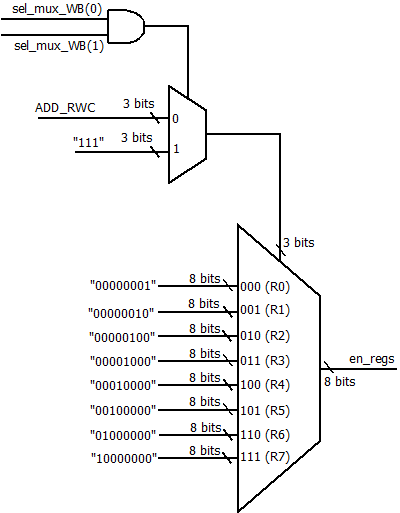
\includegraphics[keepaspectratio=true, scale=0.6]{imagens/WB2}
	\caption{Ideia original para o MUX de selecção do sinal que controla os \textit{enables} dos registos do banco de registos.}
	\vspace{-0.8em}
\end{figure}

No entanto, a solução acima tem um problema - suponha-se o caso da instrução \texttt{1401} (HEX) que corresponde a um \textit{jump if true} mediante a condição do resultado da ALU ser negativo. Os \textit{bits} \texttt{11} a \texttt{13} da instrução são \texttt{010} e, como tal, o \textit{enable} do registo \texttt{R2} ficaria activo. Porém, não se pretende escrever nesse registo. O mesmo decorre para uma operação de \textit{store} na RAM e NOP. 

Assim, para resolver o problema é necessário criar um sinal que faça \textit{overwrite} ao \textit{enable} que o MUX colocou a \textit{high}, permitindo o sinal de \textit{overwrite} colocar o \textit{enable} a \textit{low}, tal como pretendido, para que não se escreva em nenhum registo. De notar que este sinal corresponde àquele único que não é descodificado no andar de ID, decisão tomada para que os sinais que controlam a escrita no banco de registos possam estar no andar de WB, andar que corresponde de facto à escrita do resultado final.

O sinal de \textit{overwrite} foi obtido com recurso à seguinte tabela.

\vspace{1.5mm}
\begin{table}[h]
	\centering
	\caption{Sinais que permitem obter o sinal de \textit{overwrite} pretendido para cada operação.}
	\vspace{-2mm}
 	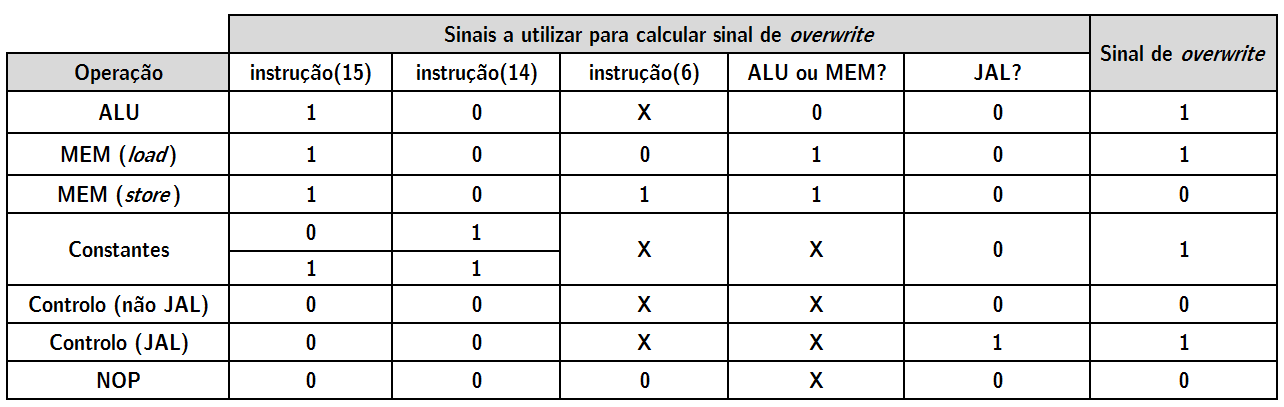
\includegraphics[keepaspectratio=true, scale=0.40]{tabelas/tabelaWE}
\end{table}

A lógica que permite implementar o sinal é demonstrada na figura seguinte.

\begin{figure}[h]
	\centering
	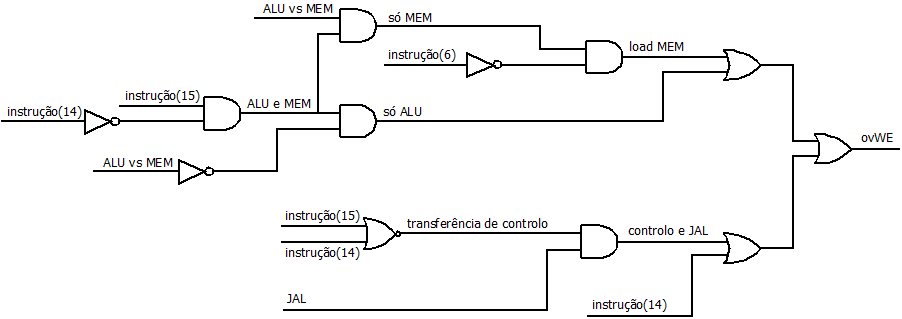
\includegraphics[keepaspectratio=true, scale=0.5]{imagens/WB3}
	\caption{Lógica que permite calcular o sinal de \textit{overwrite}.}
	\vspace{-0.8em}
\end{figure}

Como se pode ver, para o caso de operações da ALU, operações de \textit{load}, carregamento de constantes e o caso de \textit{jump and link}, o sinal de \textit{overwrite} fica a \textit{high}. Para o caso de \textit{store} na memória, transferências de controlo que não \textit{jump and link} e NOP, o sinal de \textit{overwrite} fica a \textit{low}, tal como pretendido. De notar também que a escrita nos registos é feita no flanco positivo do relógio. 

Na figura abaixo encontra-se o esquema completo do andar de \textit{write back}.

\begin{figure}[h]
	\centering
	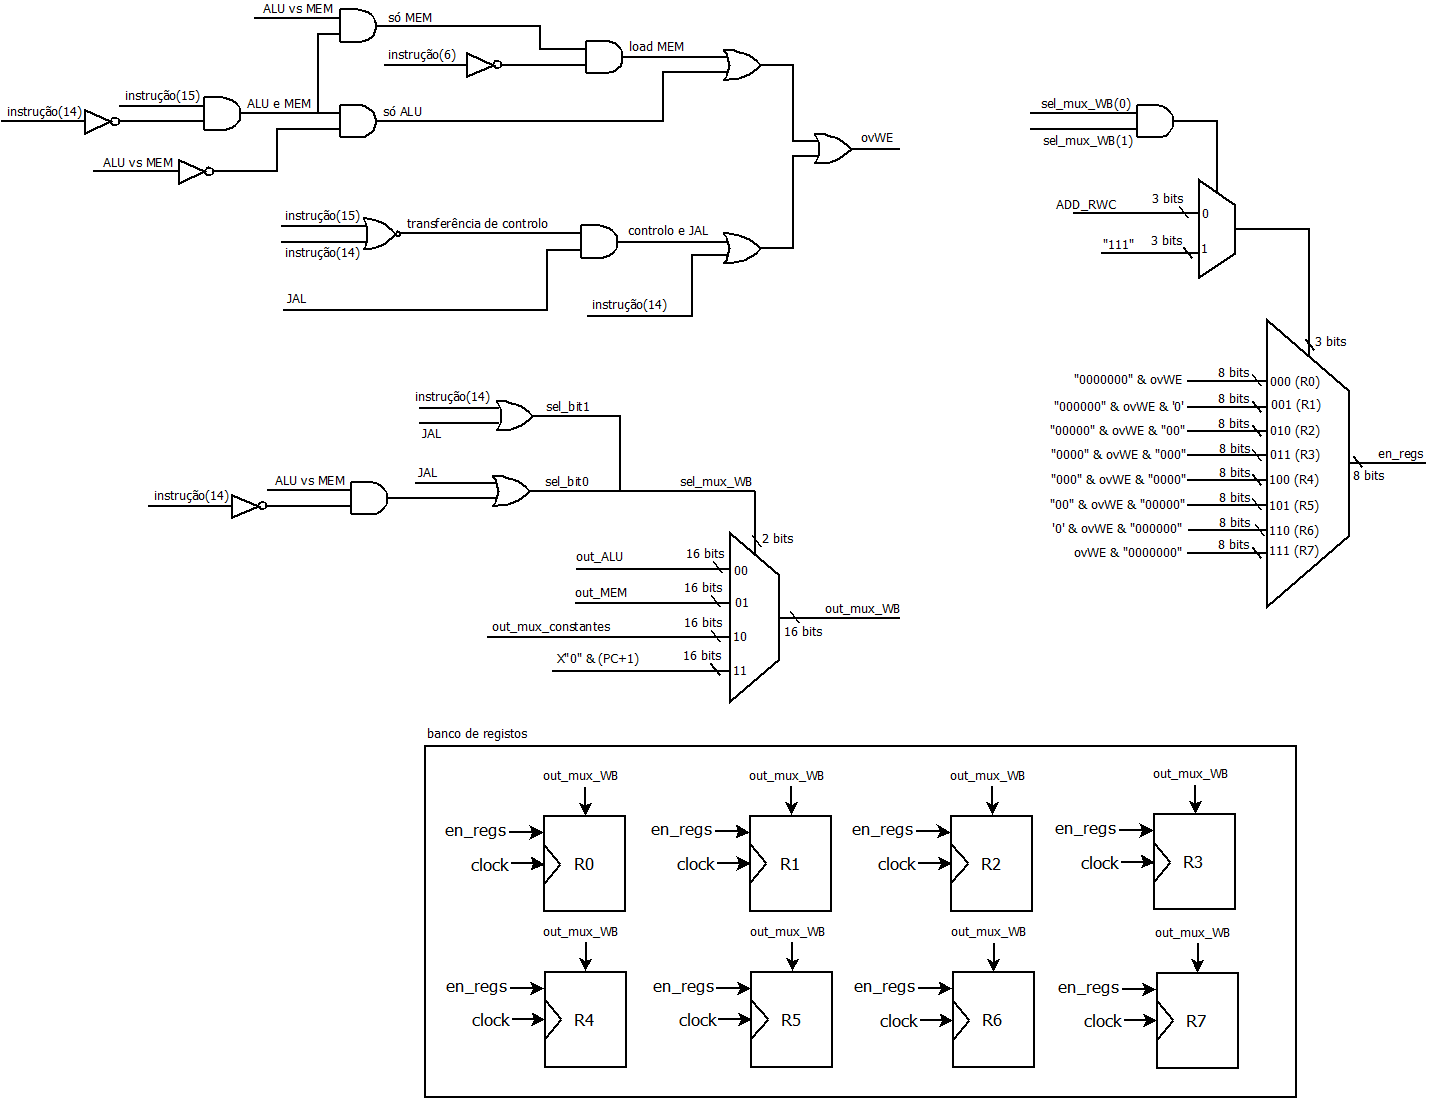
\includegraphics[keepaspectratio=true, scale=0.33]{imagens/WB}
	\caption{Esquema que representa o andar de WB e o banco de registos.}
	\vspace{-0.8em}
\end{figure}

\section{Controlo do Processador}

\todo{explicar ai os registos entre andares e maquina de estados}

\section{Conclusões}

\pagebreak

\listoftodos

\end{document}